\documentclass{standalone}
\usepackage{tikz}
\usetikzlibrary{patterns, positioning}


\begin{document}
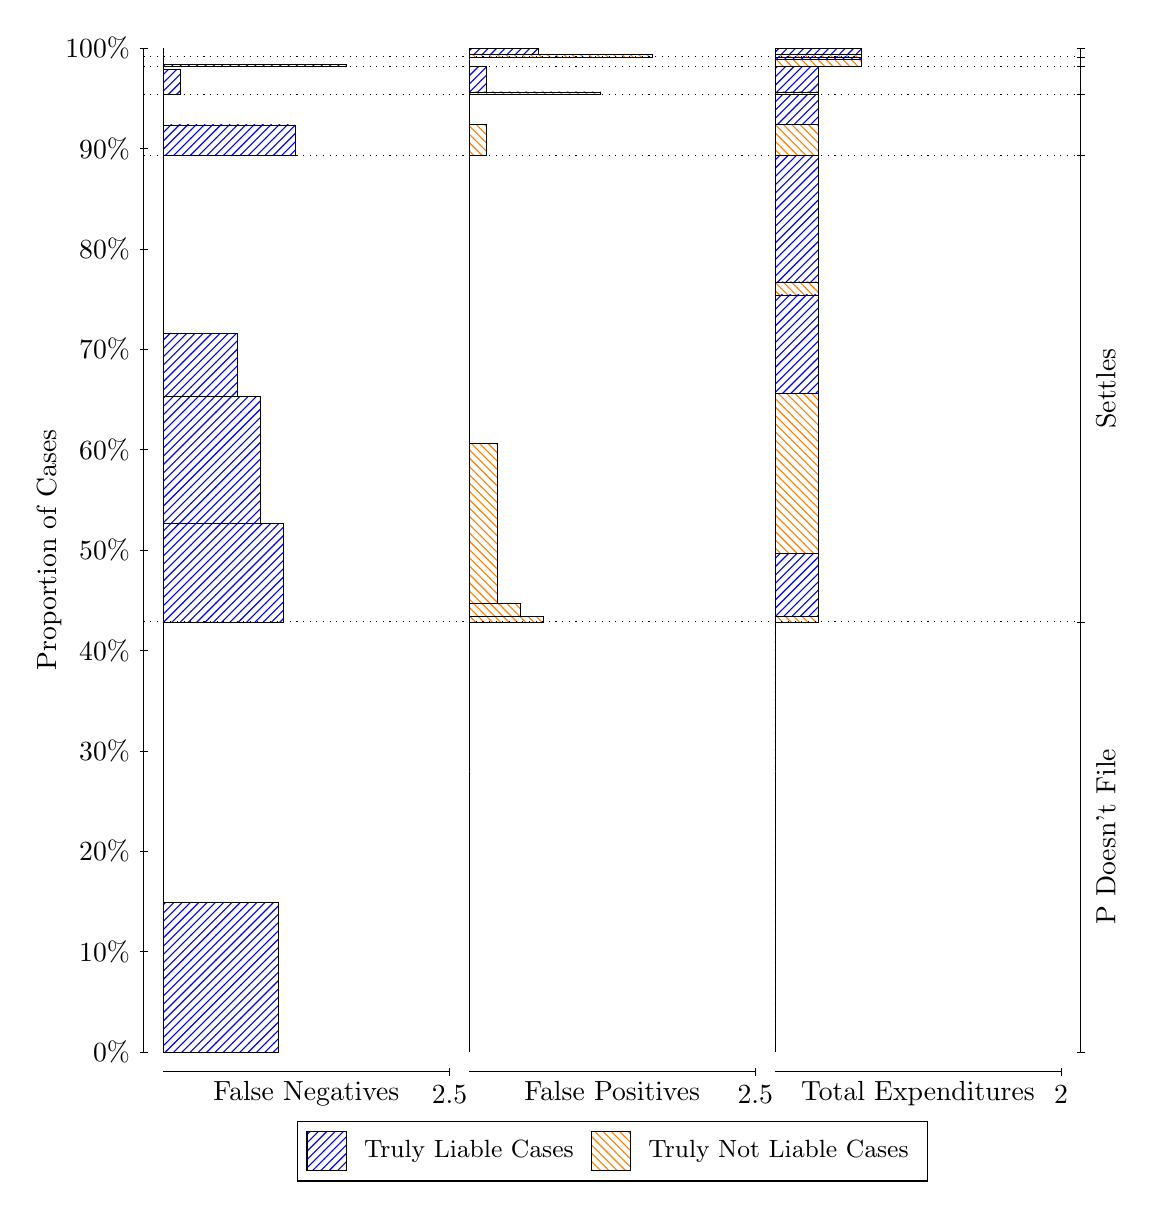
\begin{tikzpicture}
\draw[black, very thin] (1.5,1.75) -- (1.5,14.5);
\node[rotate=90, text=black, anchor=center] at (0.3, 8.125) {Proportion of Cases};
\draw[black, very thin] (1.45,1.75) -- (1.55,1.75);
\node[text=black, anchor=east] at (1.45, 1.75) {0\%};
\draw[black, very thin] (1.45,3.025) -- (1.55,3.025);
\node[text=black, anchor=east] at (1.45, 3.025) {10\%};
\draw[black, very thin] (1.45,4.3) -- (1.55,4.3);
\node[text=black, anchor=east] at (1.45, 4.3) {20\%};
\draw[black, very thin] (1.45,5.575) -- (1.55,5.575);
\node[text=black, anchor=east] at (1.45, 5.575) {30\%};
\draw[black, very thin] (1.45,6.85) -- (1.55,6.85);
\node[text=black, anchor=east] at (1.45, 6.85) {40\%};
\draw[black, very thin] (1.45,8.125) -- (1.55,8.125);
\node[text=black, anchor=east] at (1.45, 8.125) {50\%};
\draw[black, very thin] (1.45,9.4) -- (1.55,9.4);
\node[text=black, anchor=east] at (1.45, 9.4) {60\%};
\draw[black, very thin] (1.45,10.675) -- (1.55,10.675);
\node[text=black, anchor=east] at (1.45, 10.675) {70\%};
\draw[black, very thin] (1.45,11.95) -- (1.55,11.95);
\node[text=black, anchor=east] at (1.45, 11.95) {80\%};
\draw[black, very thin] (1.45,13.225) -- (1.55,13.225);
\node[text=black, anchor=east] at (1.45, 13.225) {90\%};
\draw[black, very thin] (1.45,14.5) -- (1.55,14.5);
\node[text=black, anchor=east] at (1.45, 14.5) {100\%};

\draw[black, very thin] (13.4,1.75) -- (13.4,14.5);
\draw[black, very thin] (13.35,1.75) -- (13.45,1.75);
\node[anchor=west] at (13.35, 1.75) {};
\draw[black, very thin] (13.35,7.2129) -- (13.45,7.2129);
\node[anchor=west] at (13.35, 7.2129) {};
\draw[black, very thin] (13.35,13.14) -- (13.45,13.14);
\node[anchor=west] at (13.35, 13.14) {};
\draw[black, very thin] (13.35,13.909) -- (13.45,13.909);
\node[anchor=west] at (13.35, 13.909) {};
\draw[black, very thin] (13.35,14.264) -- (13.45,14.264);
\node[anchor=west] at (13.35, 14.264) {};
\draw[black, very thin] (13.35,14.387) -- (13.45,14.387);
\node[anchor=west] at (13.35, 14.387) {};
\draw[black, very thin] (13.35,14.5) -- (13.45,14.5);
\node[anchor=west] at (13.35, 14.5) {};

\draw[black, very thin, pattern color=blue, pattern=north east lines] (1.75,1.75) rectangle (3.2033,3.6485);
\draw[black, very thin, pattern color=orange, pattern=north west lines] (1.75,3.6485) rectangle (1.75,7.2129);
\draw[black, very thin, pattern color=blue, pattern=north east lines] (1.75,7.2129) rectangle (3.276,8.4636);
\draw[black, very thin, pattern color=blue, pattern=north east lines] (1.75,8.4636) rectangle (2.9853,10.072);
\draw[black, very thin, pattern color=blue, pattern=north east lines] (1.75,10.072) rectangle (2.6947,10.873);
\draw[black, very thin, pattern color=orange, pattern=north west lines] (1.75,10.873) rectangle (1.75,13.14);
\draw[black, very thin, pattern color=blue, pattern=north east lines] (1.75,13.14) rectangle (3.4213,13.523);
\draw[black, very thin, pattern color=orange, pattern=north west lines] (1.75,13.523) rectangle (1.75,13.909);
\draw[black, very thin, pattern color=blue, pattern=north east lines] (1.75,13.909) rectangle (1.968,14.23);
\draw[black, very thin, pattern color=orange, pattern=north west lines] (1.75,14.23) rectangle (1.75,14.264);
\draw[black, very thin, pattern color=blue, pattern=north east lines] (1.75,14.264) rectangle (4.0753,14.293);
\draw[black, very thin, pattern color=orange, pattern=north west lines] (1.75,14.293) rectangle (1.75,14.387);
\draw[black, very thin, pattern color=orange, pattern=north west lines] (1.75,14.387) rectangle (1.75,14.416);
\draw[black, very thin, pattern color=blue, pattern=north east lines] (1.75,14.416) rectangle (1.75,14.5);
\draw[black, very thin, pattern color=orange, pattern=north west lines] (5.6333,1.75) rectangle (5.6333,5.3144);
\draw[black, very thin, pattern color=blue, pattern=north east lines] (5.6333,5.3144) rectangle (5.6333,7.2129);
\draw[black, very thin, pattern color=orange, pattern=north west lines] (5.6333,7.2129) rectangle (6.578,7.2813);
\draw[black, very thin, pattern color=orange, pattern=north west lines] (5.6333,7.2813) rectangle (6.2873,7.448);
\draw[black, very thin, pattern color=orange, pattern=north west lines] (5.6333,7.448) rectangle (5.9967,9.4801);
\draw[black, very thin, pattern color=blue, pattern=north east lines] (5.6333,9.4801) rectangle (5.6333,13.14);
\draw[black, very thin, pattern color=orange, pattern=north west lines] (5.6333,13.14) rectangle (5.8513,13.526);
\draw[black, very thin, pattern color=blue, pattern=north east lines] (5.6333,13.526) rectangle (5.6333,13.909);
\draw[black, very thin, pattern color=orange, pattern=north west lines] (5.6333,13.909) rectangle (7.3047,13.943);
\draw[black, very thin, pattern color=blue, pattern=north east lines] (5.6333,13.943) rectangle (5.8513,14.264);
\draw[black, very thin, pattern color=orange, pattern=north west lines] (5.6333,14.264) rectangle (5.6333,14.357);
\draw[black, very thin, pattern color=blue, pattern=north east lines] (5.6333,14.357) rectangle (5.6333,14.387);
\draw[black, very thin, pattern color=orange, pattern=north west lines] (5.6333,14.387) rectangle (7.9587,14.416);
\draw[black, very thin, pattern color=blue, pattern=north east lines] (5.6333,14.416) rectangle (6.5053,14.5);
\draw[black, very thin, pattern color=orange, pattern=north west lines] (9.5167,1.75) rectangle (9.5167,5.3144);
\draw[black, very thin, pattern color=blue, pattern=north east lines] (9.5167,5.3144) rectangle (9.5167,7.2129);
\draw[black, very thin, pattern color=orange, pattern=north west lines] (9.5167,7.2129) rectangle (10.062,7.2813);
\draw[black, very thin, pattern color=blue, pattern=north east lines] (9.5167,7.2813) rectangle (10.062,8.0819);
\draw[black, very thin, pattern color=orange, pattern=north west lines] (9.5167,8.0819) rectangle (10.062,10.114);
\draw[black, very thin, pattern color=blue, pattern=north east lines] (9.5167,10.114) rectangle (10.062,11.365);
\draw[black, very thin, pattern color=orange, pattern=north west lines] (9.5167,11.365) rectangle (10.062,11.531);
\draw[black, very thin, pattern color=blue, pattern=north east lines] (9.5167,11.531) rectangle (10.062,13.14);
\draw[black, very thin, pattern color=orange, pattern=north west lines] (9.5167,13.14) rectangle (10.062,13.526);
\draw[black, very thin, pattern color=blue, pattern=north east lines] (9.5167,13.526) rectangle (10.062,13.909);
\draw[black, very thin, pattern color=orange, pattern=north west lines] (9.5167,13.909) rectangle (10.062,13.943);
\draw[black, very thin, pattern color=blue, pattern=north east lines] (9.5167,13.943) rectangle (10.062,14.264);
\draw[black, very thin, pattern color=orange, pattern=north west lines] (9.5167,14.264) rectangle (10.607,14.357);
\draw[black, very thin, pattern color=blue, pattern=north east lines] (9.5167,14.357) rectangle (10.607,14.387);
\draw[black, very thin, pattern color=orange, pattern=north west lines] (9.5167,14.387) rectangle (10.607,14.416);
\draw[black, very thin, pattern color=blue, pattern=north east lines] (9.5167,14.416) rectangle (10.607,14.5);
\draw[black, dotted] (1.5,7.2129) -- (13.4,7.2129);
\draw[black, dotted] (1.5,13.14) -- (13.4,13.14);
\draw[black, dotted] (1.5,13.909) -- (13.4,13.909);
\draw[black, dotted] (1.5,14.264) -- (13.4,14.264);
\draw[black, dotted] (1.5,14.387) -- (13.4,14.387);
\draw[black, very thin] (1.75,1.5) -- (5.3833,1.5);
\node[text=black, anchor=north] at (3.5667, 1.5) {False Negatives};
\draw[black, very thin] (5.3833,1.45) -- (5.3833,1.55);
\node[text=black, anchor=north] at (5.3833, 1.45) {2.5};

\draw[black, very thin] (5.6333,1.5) -- (9.2667,1.5);
\node[text=black, anchor=north] at (7.45, 1.5) {False Positives};
\draw[black, very thin] (9.2667,1.45) -- (9.2667,1.55);
\node[text=black, anchor=north] at (9.2667, 1.45) {2.5};

\draw[black, very thin] (9.5167,1.5) -- (13.15,1.5);
\node[text=black, anchor=north] at (11.333, 1.5) {Total Expenditures};
\draw[black, very thin] (13.15,1.45) -- (13.15,1.55);
\node[text=black, anchor=north] at (13.15, 1.45) {2};

\node[text=black, centered, rotate=90] at (13.72, 4.4815) {P Doesn't File};
\node[text=black, centered, rotate=90] at (13.72, 10.176) {Settles};





\draw (7.449999999999999,1.5) node[draw=none] (baseCoordinate) {};
\begin{scope}[align=center]
        \matrix[scale=0.5, draw=black, below=0.5cm of baseCoordinate, nodes={draw}, column sep=0.1cm]{
            \node[rectangle, draw, minimum width=0.5cm, minimum height=0.5cm, pattern color=blue, pattern=north east lines] {}; &
            \node[draw=none, font=\small, text=black] (B) {Truly Liable Cases}; &
            \node[rectangle, draw, minimum width=0.5cm, minimum height=0.5cm, pattern color=orange, pattern=north west lines] {}; &
            \node[draw=none, font=\small, text=black] (B) {Truly Not Liable Cases}; \\
            };
\end{scope}

\end{tikzpicture}
\end{document}